\documentclass[tikz]{standalone}

%!TEX root = main.tex

% mytikzset
\usepackage{tikz}
\usetikzlibrary{positioning,arrows,shapes,patterns}
\usetikzlibrary{decorations.pathmorphing}
\usetikzlibrary{decorations.markings}
\usetikzlibrary{decorations.pathreplacing}
\usetikzlibrary{calc}
\usetikzlibrary{patterns}
\usetikzlibrary{decorations.markings}
\usetikzlibrary{petri}

\tikzset{
  vector/.style={thick,double,draw=black, postaction={decorate},
    decoration={markings,mark=at position .6 with {\arrow[black,scale=0.4]{triangle 45}}}},
  axial/.style={thick,double,densely dashed,draw=black, postaction={decorate},
    decoration={markings,mark=at position .6 with {\arrow[black,scale=0.4]{triangle 45}}}},
  gluon/.style={decorate, draw=black,
    decoration={coil,aspect=0.3,segment length=5pt,amplitude=3pt}},
  pseudo/.style={thick, dashed, draw=black, postaction={decorate},
    decoration={markings,mark=at position .6 with {\arrow[red,scale=0.5]{triangle 45}}}},
  scalar/.style={thick,draw=black, postaction={decorate},
    decoration={markings,mark=at position .6 with {\arrow[black,scale=0.5]{triangle 45}}}},
  cut/.style={draw=black, decorate, decoration={snake, segment length=1mm, amplitude=0.2mm}}
}

\begin{document}
  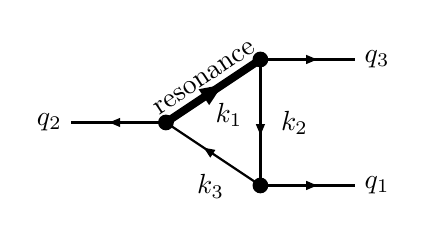
\begin{tikzpicture}[node distance=0.8cm and 1.2cm]
    \coordinate[label=left:{$q_2$}] (a1);
    \coordinate[right=of a1] (a2); \coordinate[above right=of a2]
    (b1); \coordinate[below right=of a2] (b2); \coordinate[right=of
    b1,label=right:$q_3$] (c1); \coordinate[right=of
    b2,label=right:$q_1$] (c2);

    \draw[scalar] (a2) -- (a1);
    \draw[scalar, line width=1mm] (a2) -- node[xshift=2mm, yshift=-3mm] {$k_1$} (b1);
    \draw[] (a2) -- node[above,sloped] {$\mathrm{resonance}$} (b1);
    \draw[scalar] (b2) -- node[label={below left,xshift=4mm}:$k_3$ ] {} (a2);
    \draw[scalar] (b1) -- node[label=right:$k_2$ ] {} (b2);
    \draw[scalar] (b1) -- (c1);
    \draw[scalar] (b2) -- (c2);

    \fill[black] (a2) circle (1mm);
    \fill[black] (b1) circle (1mm);
    \fill[black] (b2) circle (1mm);
  \end{tikzpicture}
\end{document}
